\documentclass[a4paper,12pt,oneside,openany]{book}	
\usepackage{layout}
\setlength{\textwidth}{15.0 cm}
\setlength{\textheight}{25.0 cm}


\usepackage[english,portuges]{babel}
\usepackage{pagina}	% pagina-padrao
\usepackage{indentfirst}		% for indent
\usepackage[latin1]{inputenc}
\usepackage{graphics,epsfig}
\usepackage{graphics}
\graphicspath{{./figuras/}}
\usepackage{pstricks,pst-node,pst-tree}
\usepackage{alltt}
%\usepackage{makeidx}
%\makeindex
\usepackage[figuresright]{rotating} % for saydways tables and figures
\usepackage{enumerate}			% for configuration of enumerate environment
\usepackage{amsmath}
\usepackage{amssymb}
\usepackage{portland,multirow}

\setcounter{secnumdepth}{3}	% numeracao ate subsubsecao
\setcounter{tocdepth}{2}	% indice ate subsubsecao

\usepackage{longtable}

%code
\usepackage{listings}

%tree structures
\usepackage{forest}

\begin{document}

\frontmatter
\thispagestyle{empty}


\includegraphics[scale=0.7]{Poli.eps}

\begin{center}
\large{FRAMEWORK PARA SERVI�OS DE APRENDIZADO DE M�QUINA}\\
   \vspace{2cm}
\large{PEDRO HOLLANDA BOUEKE}\\
\end{center}
   \vspace{3cm}
\hspace{7cm}
\hfill \parbox{8.0cm}{Projeto de Gradua��o apresentado ao Curso de Engenharia de Computa��o e Informa��o da Escola Polit�cnica, Universidade Federal do Rio de Janeiro, como parte dos requisitos necess�rios � obten��o do t�tulo de Engenheiro.\\}
   \vspace{2cm}
\hfill \parbox{8.0cm}{Orientador: Fl�vio Luis de Mello} \\
   \vspace{2cm}
\begin{center}
Rio de Janeiro

Mar�o de 2019
\end{center}




\pagebreak


\begin{center}
\large{FRAMEWORK PARA SERVI�OS DE APRENDIZADO DE M�QUINA}\\
   \vspace{1cm}
\large{PEDRO HOLLANDA BOUEKE}\\
\end{center}
   \vspace{2cm}
PROJETO DE GRADUA��O SUBMETIDO AO CORPO DOCENTE DO CURSO DE ENGENHARIA DE COMPUTA��O E INFORMA��O DA ESCOLA POLIT�CNICA DA UNIVERSIDADE FEDERAL DO RIO DE JANEIRO COMO PARTE DOS REQUISITOS NECESS�RIOS PARA A OBTEN��O DO GRAU DE ENGENHEIRO DE COMPUTA��O E INFORMA��O
   
   \vspace{1cm}
Autor:
      \vspace{0.5cm}
      \begin{flushright}
         \parbox{10cm}{
            \hrulefill

            \vspace{-.375cm}
            \centering{PEDRO HOLLANDA BOUEKE}

            \vspace{0.1cm}
         }
      \end{flushright}
      
      
Orientador:
      \vspace{0.5cm}
      \begin{flushright}
         \parbox{10cm}{
            \hrulefill

            \vspace{-.375cm}
            \centering{Fl\'avio Luis de Mello, DSc}

            \vspace{0.1cm}
         }
      \end{flushright}
      
Examinador:
      \vspace{0.5cm}
      \begin{flushright}
         \parbox{10cm}{
            \hrulefill

            \vspace{-.375cm}
            \centering{Diego Leonel Cadette Dutra, DSc}

            \vspace{0.1cm}
         }
      \end{flushright}
      
Examinador:
      \vspace{0.5cm}
      \begin{flushright}
         \parbox{10cm}{
            \hrulefill

            \vspace{-.375cm}
            \centering{Manoel Villas Boas Junior, MSc}

            \vspace{0.1cm}
         }
      \end{flushright}
      
                        
      \vfill
      
      
\begin{center}
Rio de Janeiro

Mar�o de 2019
\end{center}


\pagebreak            

% Declaracao
\begin{center}
Declara��o de Autoria e de Direitos
\end{center}

\vspace{0.5cm}

Eu, \emph{Pedro Hollanda Boueke} CPF \emph{108.243.966.50}, autor da monografia \emph{Framework para Servi�os de Aprendizado de M�quina}, subscrevo para os devidos fins, as seguintes informa��es:\\
1. O autor declara que o trabalho apresentado na disciplina de Projeto de Gradua��o da Escola Polit�cnica da UFRJ � de sua autoria, sendo original em forma e conte�do.\\
2. Excetuam-se do item 1. eventuais transcri��es de texto, figuras, tabelas, conceitos e id�ias, que identifiquem claramente a fonte original, explicitando as autoriza��es obtidas dos respectivos propriet�rios, quando necess�rias.\\
3. O autor permite que a UFRJ, por um prazo indeterminado, efetue em qualquer m�dia de divulga��o, a publica��o do trabalho acad�mico em sua totalidade, ou em parte. Essa autoriza��o n�o envolve �nus de qualquer natureza � UFRJ, ou aos seus representantes.\\
4. O autor pode, excepcionalmente, encaminhar � Comiss�o de Projeto de Gradua��o, a n�o divulga��o do material, por um prazo m�ximo de 01 (um) ano, improrrog�vel, a contar da data de defesa, desde que o pedido seja justificado, e solicitado antecipadamente, por escrito, � Congrega��o da Escola Polit�cnica.\\
5. O autor declara, ainda, ter a capacidade jur�dica para a pr�tica do presente ato, assim como ter conhecimento do teor da presente Declara��o, estando ciente das san��es e puni��es legais, no que tange a c�pia parcial, ou total, de obra intelectual, o que se configura como viola��o do direito autoral previsto no C�digo Penal Brasileiro no art.184 e art.299, bem como na Lei 9.610.\\
6. O autor � o �nico respons�vel pelo conte�do apresentado nos trabalhos acad�micos publicados, n�o cabendo � UFRJ, aos seus representantes,  ou ao(s) orientador(es), qualquer responsabiliza��o/ indeniza��o nesse sentido.\\
7. Por ser verdade, firmo a presente declara��o.\\

      \vspace{0.5cm}
      \begin{flushright}
         \parbox{10cm}{
            \hrulefill

            \vspace{-.375cm}
            \centering{Pedro Hollanda Boueke}

            \vspace{0.1cm}
         }
      \end{flushright}
      
\pagebreak

% Copyright
      \vspace{0.5cm}

UNIVERSIDADE FEDERAL DO RIO DE JANEIRO \\
Escola Polit�cnica - Departamento de Eletr�nica e de Computa��o \\
Centro de Tecnologia, bloco H, sala H-217, Cidade Universit�ria \\ 
Rio de Janeiro - RJ      CEP 21949-900\\
\vspace{0.5cm}
\paragraph{}Este exemplar � de propriedade da Universidade Federal do Rio de Janeiro, que poder� inclu�-lo em base de dados, armazenar em computador, microfilmar ou adotar qualquer forma de arquivamento.
\paragraph{}� permitida a men��o, reprodu��o parcial ou integral e a transmiss�o entre bibliotecas deste trabalho, sem modifica��o de seu texto, em qualquer meio que esteja ou venha a ser fixado, para pesquisa acad�mica, coment�rios e cita��es, desde que sem finalidade comercial e que seja feita a refer�ncia bibliogr�fica completa.
\paragraph{}Os conceitos expressos neste trabalho s�o de responsabilidade do(s) autor(es).


\pagebreak

 Dedicat�ria
\begin{center}
\textbf{DEDICAT�RIA}
\end{center}
      \vspace{0.5cm}

\paragraph{}Dedico todo o esfor�o relacionado ao trabalho aqui exposto, bem como todos os meus anos de estudo e forma��o, � minha m�e, que fez de tudo em sua vida para me fornecer a melhor educa��o que p�de, mas se foi antes de presenciar esse momento. Serei eternamente grato pelo seu amor.

\pagebreak


% Agradecimento
\begin{center}
\textbf{AGRADECIMENTO}
\end{center}
      \vspace{0.5cm}

\paragraph{}Agrade�o a todas as pessoas presentes durante a minha jornada acad�mica, em especial ao professor Fl�vio Luis de Mello. Agrade�o tamb�m ao povo brasileiro, que contribuiu de forma significativa � minha forma��o e estada nesta Universidade. Este projeto � uma pequena forma de retribuir o investimento e confian�a em mim depositados. 

\pagebreak


% Resumo
\begin{center}
\textbf{RESUMO}
\end{center}
      \vspace{0.5cm}

\paragraph{}O trabalho aqui exposto tem como finalidade propor uma plataforma para execu��o de modelos de aprendizado de m�quina de forma escalonada e de f�cil ger�ncia, se tratando de um sistema configur�vel e acess�vel a usu�rios por meio de uma interface \textit{web}. O trabalho aborda a arquitetura desse sistema e uma implementa��o e implanta��o, apresentando suas componentes, funcionamento e um prot�tipo para sua valida��o. Tamb�m s�o realizadas conclus�es em cima do trabalho desenvolvido e s�o apresentados trabalhos futuros em cima da proposta exposta.
\paragraph{}
\noindent Palavras-Chave: aprendizado de m�quina, django, agendador de tarefas, aplica��o \textit{web}.

\pagebreak


% Abstract
\begin{center}
\textbf{ABSTRACT}
\end{center}
      \vspace{0.5cm}

\paragraph{}The work here shown has the aim of proposing a framework for the execution of machine learning models in a easily managed and scalable manner, constituted by a configurable system accessible by users by the way of a web interface. The work approaches this system's architecture, an implementation and a deployment, going through its components, its functioning and a prototype for validation of the project. It also elaborates conclusions over the developed work and apresents future work propositions.
\paragraph{}
\noindent Key-words: machine learning, django, job sheduler, web application.

\pagebreak


% Siglas
\begin{center}
\textbf{SIGLAS}
\end{center}
      \vspace{0.5cm}

\paragraph{}AWS - Amazon Web Services
\paragraph{}HTML - Hypertext Markup Language
\paragraph{}MTV - Model Template View
\paragraph{}ODBC - Open Database Connectivity
\paragraph{}UFRJ - Universidade Federal do Rio de Janeiro 

%\paragraph{}WYSIWYG - \textit{What you see is what you get} 


\pagebreak









% Table of Contents
% ---------------------------------------------------------------
\tableofcontents
% ---------------------------------------------------------------
% Lista de figuras
% ---------------------------------------------------------------
%\cleardoublepage
%\addcontentsline{toc}{chapter}{Lista de Figuras}
\listoffigures
% ---------------------------------------------------------------
% Lista de Tabelas
% ---------------------------------------------------------------
%\cleardoublepage
%\addcontentsline{toc}{chapter}{Lista de Tabelas}
\listoftables

\mainmatter
\cleardoublepage
% ---------------------------------------------------------------
% Chapter 1 - Introdu��o
% ---------------------------------------------------------------
\chapter{Introdu��o}
\label{cap1}
\section{Tema}

\paragraph{}O trabalho apresenta uma solu��o para uma das quest�es comumente negligenciadas dentro da �rea de tecnologias de Aprendizado de M�quina: a implanta��o e uso de modelos em ambientes n�o acad�micos. A proposta executada se reserva � cria��o de um \textit{framework} para ger�ncia e execu��o de modelos de Aprendizado de M�quina de forma a automatizar os processos relacionados ao uso de tais modelos, da coleta dos dados a serem analisados, passando por sua execu��o at� a entrega dos resultados.

\paragraph{}Nesse trabalho s�o abordados princ�pios de Engenharia de Software, algoritmos de Aprendizado de M�quina, \textit{Job Schedulers} e desenvolvimento de aplica��es web com a plataforma de desenvolvimento \textit{Django}. Objetiva-se a cria��o de uma plataforma gen�rica para a execu��o peri�dica de modelos de Aprendizado de M�quina que permita o acompanhamento da execu��o e resultados por diversos usu�rios, tamb�m facilitando a reconfigura��o de agendas e ger�ncia do \textit{workflow} de processamento em ambientes de produ��o.

%\paragraph{}Falar do que se trata o trabalho usando uma vis�o macrosc�pica (tamanho do texto: 1 ou 2 par�grafos no m�ximo).

%\paragraph{}Sobre que grande �rea de conhecimento voc� vai falar?

%\paragraph{}Dada esta grande �rea, qual � o subconjunto de conhecimento sobre o qual ser� o seu trabalho?

%\paragraph{}Qual o problema a ser resolvido?


\section{Delimita��o}

\paragraph{}O trabalho apresentado se destina a atender as demandas de agentes de todas as esferas do c�rculo de usu�rios de modelos de Aprendizado de M�quina. Enquanto necess�rias execu��es recorrentes de modelos, o \textit{framework} desenvolvido apresenta uma solu��o compat�vel aos principais contextos em que tais modelos se apresentam. S�o exce��es not�veis a esse conjunto de usu�rios parte dos desenvolvedores de modelos de Aprendizado de M�quina que, possivelmente, n�o estejam interessados em praticar execu��o de seus modelos em ambientes de produ��o. Tamb�m se excluem aqueles que n�o possuem requisitos t�cnicos para a execu��o dos componentes necess�rios ao sistema, como usu�rios do sistema operacional Windows, usu�rios de bancos de dados incompat�veis com a linguagem SQL e usu�rios impossibilidatos de fazer uso da linguagem de programa��o \textit{Python 3}.

%\paragraph{}Realizar uma delimita��o informando de quem � a demanda, em que local, e em que momento no tempo. Eventualmente, pode ser mais f�cil come�ar pensando por exclus�o, ou seja, para quem n�o serve, onde n�o deve ser aplicado, e em seguida pegar o universo que sobra (tamanho do texto: livre).


\section{Justificativa}

\paragraph{} Enquanto que algoritmos e modelos matem�ticos s�o apresentados frequentemente pelo ambiente acad�mico como solu��es aproximadas de problemas reais e complexos condizentes ao que se diz respeito da �rea de Aprendizado de M�quina, a sua implanta��o em ambientes n�o acad�micos ou de produ��o poucas vezes � abordada. Dado esse cen�rio, nota-se que existe espa�o e demanda para o estudo e desenvolvimento de novas metodologias e plataformas que ambicionem solu��es para as dificuldades envolvidas em trazer um modelo de Aprendizado de M�quina para um ambiente n�o acad�mico, dentre as quais destacam-se: ger�ncia de execu��es e processamento, ger�ncia de arquivos e modelos, visualiza��o e acompanhamento de resultados. 

%\paragraph{}Apresentar o porqu� do tema ser interessante de ser estudado. Cuidado, n�o � a motiva��o particular. Devem ser apresentadas raz�es para que algu�m deva se %interessar no assunto, e n�o quais foram suas raz�es particulares que motivar.am voc� a estud�-lo (tamanho do texto: livre).


\section{Objetivos}

\paragraph{} Objetiva-se o desenvolvimento de um \textit{framework} que permita o agendamento e acompanhamento de execu��es de modelos de Aprendizado de M�quina. Uma execu��o caracteriza-se pela instancia��o de um modelo, coleta dos dados a serem processados, execu��o do modelo sobre os dados coletados e persist�ncia tanto dos resultados quanto das informa��es relativas � execu��o. Por acompanhamento, refere-se � possibilidade de usu�rios do \textit{framework} visualizarem os resultados das execu��es, bem como de configurarem todos os aspectos da execu��o, como a agenda, o modelo e as bases de persist�ncia.

\paragraph{}O acima descrito ser� alcan�ado com a implementa��o bem sucedida de um \textit{framework} que permita que todos os detalhes descritos sejam executados, fazendo uso de um sistema de agendamento de tarefas para agendamento de execu��es do modelo; uma plataforma de desenvolvimento de aplica��es web para permitir o acompanhamento e ger�ncia das execu��es; bases de dados que contenham as informa��es dos usu�rios do sistema, registros detalhando as etapas das execu��es do modelo e os dados a serem processados. Dessa forma, ser�o objetivos parciais para se alcan�ar o fim desejado:

\begin{enumerate}
\item Desenvolvimento de uma aplica��o web caracterizada por:
\begin{enumerate}
\item Permitir agendamento de execu��es de programas para processamento de modelos de Aprendizado de M�quina.
\item Permitir a visualiza��o de resultados e eventos gerados pelos processos agendados.
\item Se comunicar com bases de dados externas para coleta e persist�ncia de dados.
\item Ser reconfigur�vel a fim de atender ambientes diversos.
\end{enumerate}
\item Desenvolvimento de uma base de dados relacionais para armazenamento de eventos do \textit{framework}.
\item Desenvolvimento de um programa agend�vel para execu��o de modelos de Aprendizado de M�quina.
\end{enumerate}

%\paragraph{}Informar qual � o objetivo geral do trabalho, isto �, aquilo que deve ser atendido e que corresponde ao indicador inequ�voco do sucesso do seu trabalho. Pode acontecer que venha a existir um conjunto de objetivos espec�ficos, que complementam o objetivo geral (tamanho do texto: livre, mas cuidado para n�o fazer uma literatura romanceada, afinal esta se��o trata dos objetivos).


\section{Metodologia}

\paragraph Atendendo �s expectativas de um projeto de \textit{Software}, iniciou-se o projeto a partir de diagramas e modelos de Engenharia de Software que definem o funcionamento do sistema projetado. Foram elaborados: um diagrama de casos de uso, um diagrama de sequ�ncia, cinco diagramas de atividade e um diagrama de relacionamento de entidades.

\paragraph{}Com o planejamento te�rico conclu�do, foram definidas as ferrametnas de desenvolvimento do sistema. Para controle de vers�o foi utilizada a ferramenta \textit{Git}, com a manuten��o de um reposit�rio para todo o c�digo produzido. Como linguagem de desenvolvimento, foi escolhida a linguagem \textit{Python 3}, que se destaca por ser uma das principais linguagens de programa��o dentro da comunidade de particantes de Aprendizado de M�quina \cite{StackSurvey18}.

%\paragraph{}Como � a abordagem do assunto. Como foi feita a pesquisa, se vai houve valida��o, etc. Em resumo, voc� de explicar qual foi sua estrat�gia para atender ao objetivo do trabalho (tamanho do texto: livre).


\section{Descri��o}

%\paragraph{}No cap�tulo 2 ser� .....

%\paragraph{}O cap�tulo 3 apresenta ...

%\paragraph{}Os .... s�o apresentados no cap�tulo 4. Nele ser� explicitado ...

%\paragraph{}E assim vai at� chegar na conclus�o.


% ---------------------------------------------------------------
% Chapter 2 - Informa��es Adicionais
% ---------------------------------------------------------------
\chapter{Fundament��o Te�rica}
\label{cap2}
\section{Sistemas de Aprendizado de M�quina em Ambiente de Produ��o}

\paragraph{}Sistemas de Aprendizado de M�quina s�o sistemas que combinam algoritmos e modelos matem�ticos da �rea de Aprendizado de M�quina em solu��es que visam a implanta��o do uso de tais algoritmos e modelos em ambientes reais. Aprendizado de m�quina, por sua vez, se refere a �rea de estudos voltata ao desenvolvimento e compreens�o de modelos matem�ticos caracterizados pelo aprimoramento de seus resultados por meio da ingest�o de dados de treino, de forma que esses modelos possam realizar predi��es e decis�es sem que sejam explicitamente programados para o fazerem, como aponta Christopher Bishop \cite{Bishop}.

\paragraph{}No passado, a aplica��o de tecnologias de Aprendizado de M�quina era limitada pela baixa capacidade computacional e pela necessidade de grandes massas de dados, que n�o eram coletadas e armazenadas. Com a populariza��o da computa��o, por conta do fen�meno de escala, o campo se tornou um foco para o surgimento de novas tecnologias que se apresentam, em grande parte, como inova��es na academia e n�cleos de pesquisa. O surgimento de novos paradigmas no campo n�o se viu acompanhado, em mesma escala, pelo surgimento de novos sistemas e metodologias de implanta��o das novas tecnologias em ambientes n�o acad�micos.

\paragraph{}Enquanto que modelos tomadores de decis�es dominam a �rea, sistemas que permitiriam a implanta��o de tais modelos em ambientes de produ��o se encontram pouco difundidos. Atualmente, os principais sistemas desse tipo se encontram hospedados em solu��es prontas por provedores de infra-estrutura gerenciada, como � o caso do \textit{Amazon SageMaker} e do \textit{Machine Learning Studio}, solu��es pagas providenciadas pela \textit{AWS} e pela \textit{Azure}, respectivamente. Em contrapartida, solu��es abertas e gratuitas ainda dependem de um grande trabalho de desenvolvimento por parte dos respons�veis pela implanta��o, requerendo um esfor�o similar ao desenvolvido no trabalho aqui exposto.

\section{Agendadores de Tarefas}


\paragraph{}Para a implanta��o de um sistema de \textit{stream} de dados para processamento constante, � necess�ria uma forma para a inicializa��o da execu��o de programas e tarefas correlatas ao trabalho sendo executado. Nesse sentido, considera-se �teis ferramentas agendadoras de tarefas, ou \textit{job shedulers}. Essas s�o ferramentas respons�veis pela execu��o agendada de programas, viabilizando metas de frequencia de processamento e execu��o.

\subsection{Slurm}

\paragraph{}Uma dessas ferramentas � o programa conhecido por \textit{slurm} \cite{Slurm}, um \textit{workload manager} capaz de realizar o agendamento de tarefas. Essa � uma das principais ferramentas de c�digo aberto utilizada em sistemas \textit{Unix-like}, capaz de funcionar em \textit{clusters} computacionais de forma distribu�da ou baseada em apenas um inst�ncia. O Slurm n�o requer modifica��es no \textit{kernel} do sistema operacional, sendo relativamente auto contido por conta disso.

\paragraph{}As tr�s principais fun��es do \textit{slurm} s�o a aloca��o de recursos de maneira exclusiva e n�o exclusiva a usu�rios por um per�odo de tempo; prover um \textit{framework} para iniciar, executar e monitorar tarefas paralelas em um conjunto de n�s computacionais; arbitrar a conten��o de recursos gerenciando filas de trabalhos pendentes. Sua arquitetura consiste de um daemon rodando em cada n� e um daemon central no n� principal. Os daemons prov�m comunica��o hier�rquica tolerante a falhas.

\paragraph{}Os n�s da rede se dividem em parti��es, cada uma sendo uma fila de tarefas, cada tarefa � subdividida em subtarefas, que podem ser processadas pela parti��o em paralelo. Uma vez alocada a um conjunto de n�s, o usu�rio � capaz de iniciar o trabalho em paralelo no forma de subtarefas em qualquer configura��o dentro da aloca��o de n�s.

\subsection{Crontab}

\paragraph{}Outra ferramenta dessa categoria, a utilizada nesse trabalho, � o \textit{crontab} \cite{Crontab}. O nome � uma abrevia��o de \textit{cron table}, pois se refere ao arquivo \textit{cron file} utilizado internamente para agendamento e execu��o de tarefas. Esse programa consiste de um arquivo no sistema operacional que periodicamente � lido pelo \textit{cron} daemon, fazendo uso de express�es \textit{CRON}, e suas linhas s�o interpretadas como entradas de uma tabela contendo em uma coluna a express�o que define sua agenda de execu��o e em outra coluna o comando a ser executado como um programa de linha de comando. Seu diferencial est� no fato de ser extremamente simples e possuir suporte para manipula��o por meio de diversas linguagens de programa��o, incluindo \textit{Python 3}, a linguagem escolhida para o desenvolvimento do sistema aqui detalhado.

\section{Desenvolvimento com Django}

\paragraph{}O \textit{Django} \cite{Django} � um \textit{framework} de desenvolvimento de aplica��es e servi�os \textit{web} dispon�vel nas linguagens de programa��o \textit{Python 2 e 3}, gratuito e de c�digo aberto. Sua estrutura interna � baseada no paradigma MTV, particularmente caracterizada por uma forte e nativa integra��o com bancos de dados a partir de uma interface pr�pria. Todos os componentes de uma aplica��o \textit{web} s�o reproduzidos por meio de conven��es pr�prias ao \textit{framework}, baseados na reusabilidade de c�digo e orientado � integra��o nativa com bancos de dados diversos.

\paragraph{}O desenvolvimento com o \textit{framework} � marcado pela pouca quantidade de c�digo produzido e pelas diversas interfaces de programa��o providas pela plataforma. Tamb�m se destacam a a integra��o nativa com um sistema de administra��o embutido nas aplica��es produzidas que fornecem, sem custos adicionais de desenvolvimento, uma aplica��o e interface de autentica��o de usu�rios tamb�m utiliz�vel em todas as camadas de servi�o contru�das paralelamente no mesmo ambiente.

\paragraph{}O \textit{framework} disponibiliza ao desenvolvedor interfaces pr�prias para o acesso a bancos de dados, templates para renderiza��o de HTML, classes extens�veis para programa��o orientada a objetos, encaminhamento de requisi��es configur�vel, dentre outras facilidades.

\section{Amazon AWS}

\paragraph{} A \textit{Amazon Web Services}, ou AWS, � a maior provedora de infraestrutura em nuvem do mercado. A empresa prov� servi�os para websites, aplica��es cliente servidor, banco de dados, an�lise de dados, redes, dispositivos m�veis, ferramentas de gerenciamento, armazenamento de dados, aluguel de servidores entre outros \cite{AWS}. Seus servi�os podem ser acessados em seu portal \textit{web} e por meio de suas \textit{API}s e \textit{SDK}s.

\paragraph{} A Amazon est� dispon�vel em diversas localidades, operando \textit{datacenters} ao redor do mundo. Cada local � composto por uma regi�o e zonas de disponibilidade, onde uma regi�o � uma zona geogr�fica totalmente independente das demais, contendo diversas zonas de disponibilidade tamb�m isoladas entre si. A AWS adota, para a maioria de seus servi�os, o plano de pagamento \textit{pay-as-you-go} \cite{AWSpay}, fazendo necess�rio apenas o pagamento pelos recusrsos consumidos.

% ---------------------------------------------------------------
% Chapter 3 - Implementa��o
% ---------------------------------------------------------------
\chapter{Proposta de Plataforma}
\label{cap3}
\section{Arquitetura}

\paragraph{}O projeto desenvolvido se trata de uma aplica��o \textit{Django} que conta com tr�s interfaces, uma para execu��o de um modelo preditivo em ocorr�ncias controladas, outra para monitoramento dos servi�os associados e outra para a visualiza��o dos resultados das predi��es, chamadas, respectivamente, de \textit{Showroom}, \textit{Monitor} e \textit{Disparo}. Essas tr�s interfaces s�o controladas pela aplica��o por meio de tr�s classes, vistas na figura 3.1. Os componentes da aplica��o podem ser visualizados na figura 3.2, onde se observa a exist�ncia de um arquivo \textit{config.yaml}, respons�vel por agregar todos os par�metros e configura��es da aplica��o.

Al�m da aplica��o, existem as componentes \textit{daemon.py} e \textit{datalake.py} que s�o respons�veis, respectivamente, pela predi��o de resultados e conex�o com o \textit{datalake} onde est�o os dados a sofrerem predi��es. O escalonamento de predi��es � gerenciado pelo \textit{crontab}, que, por sua vez, � gerenciado pela aplica��o.


\section{Implementa��o}

\paragraph{} No modelo seguido pelo \textit{framework Django}, o modelo \textit{MTV}, todas as p�ginas e interfaces da aplica��o s�o renderizadas a partir de templates HTML preenchidos pelo controlador da aplica��o, que no caso se trata do arquivo \textit{views.py}. Os templates HTML se encontram dentro do diret�rio \textit{templates}. Os modelos se encontram no arquivo \textit{models.py}, fazendo uso direto das classes de modelo do \textit{framework}. As rotas da aplica��o se encontram no arquivo \textit{urls.py}. As componentes \textit{monitor.py}, \textit{showroom.py}, \textit{dispatch.py}, \textit{datalake.py} e \textit{daemon.py} se encontram no diret�rio \textit{scripts}.

\begin{figure}
\begin{center}
\parbox[htb]{13.0cm}
  {
  \begin{center}
  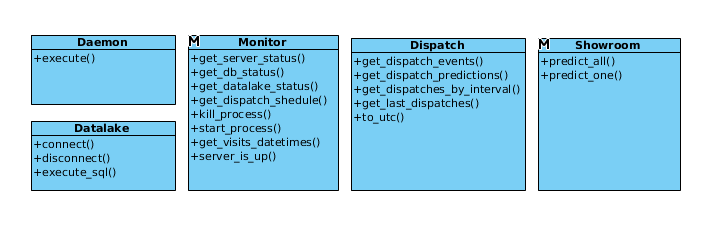
\includegraphics[scale=0.5]{framework_clases.png}
  \caption[\small{Diagrama de classes da aplica��o.}]{\label{FigDel} \small{Diagrama de classes da aplica��o.}}
  \end{center}
  }
\end{center}
\end{figure}

\begin{figure}
\begin{center}
\parbox[htb]{13.0cm}
  {
  \begin{center}
  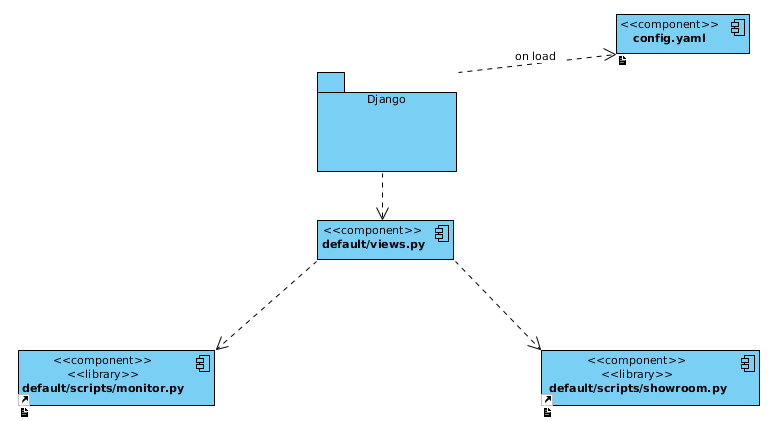
\includegraphics[scale=0.50]{framework.png}
  \caption[\small{Diagrama de componentes da aplica��o.}]{\label{FigDel} \small{Diagrama de componentes da aplica��o.}}
  \end{center}
  }
\end{center}
\end{figure}

\subsection{Configura��o}

\paragraph{}Toda a configura��o da aplica��o � feita a partir de dois arquivos, o \textit{settings.py} e o \textit{config.yaml}. No primeiro s�o configuradas as propriedades b�sicas de uma aplica��o \textit{Django}, se tratando de seu arquivo de configura��o padr�o. No segundo, est�o as configura��es espec�ficas a essa aplica��o. O caminho ao arquivo \textit{config.yaml} � escrito como a vari�vel \textit{CONFIG\_FILE}, dentro do arquivo \textit{settings.py}, para que as configura��es possam ser carregadas na aplica��o durante sua inicializa��o.

% Please add the following required packages to your document preamble:
% \usepackage{graphicx}
\begin{table}[]
\caption{Par�metros de configura��o contidos no arquivo \textit{config.yaml}.}
\centering
\resizebox{\textwidth}{!}{%
\begin{tabular}{|l|l|}
\hline
Par�metro                                   & Descri��o                                                                                                                                                                                     \\ \hline
monitor.controllerserver.address            & Endere�o (ip ou nome de dom�nio) para o servidor monitorado                                                                                                                                   \\ \hline
monitor.controller.server.machanism         & \begin{tabular}[c]{@{}l@{}}Mecanismo de conex�o  com o servidor monitorado (plain ou ssl para ips,\\  dns para nomes de dom�nio)\end{tabular}                                                 \\ \hline
monitor.controller.server.port              & Porta de conex�o com o servidor monitorado(apenas para ips)                                                                                                                                   \\ \hline
monitor.view.refresh\_rate                  & Segundos entre atualiza��es das informa�oes na view monitor                                                                                                                                   \\ \hline
dispatch.view.filter.default\_offset        & Diferen�a temporal padr�o para o filtro de disparos                                                                                                                                           \\ \hline
showroom.controller.max\_min\_model\_path   & Arquivo de modelo usado para pr�-tratamento das amostras                                                                                                                                      \\ \hline
showroom.controller.prediction\_model\_path & Arquivo de modelo usado para a predi��o dos resultados                                                                                                                                        \\ \hline
showroom.controller.samples\_path           & Arquivo contendo amostras em formato csv                                                                                                                                                      \\ \hline
showroom.controller.number\_of\_columns     & N�mero de colunas entre as primeiras do arquivo a serem mostradas na view                                                                                                                     \\ \hline
mysql\_events\_db.name                      & Nome do banco de eventos                                                                                                                                                                      \\ \hline
mysql\_events\_db.user                      & Nome do usu�rio do banco de dados                                                                                                                                                             \\ \hline
mysql\_events\_db.password                  & Senha do usu�rio do banco de enventos                                                                                                                                                         \\ \hline
mysql\_events\_db.host                      & Endere�o do banco de eventos                                                                                                                                                                  \\ \hline
mysql\_events\_db.port                      & Porta de acesso ao banco de eventos                                                                                                                                                           \\ \hline
datalake.connection\_string                 & Cadeia de conex�o ODBC para o datalake                                                                                                                                                        \\ \hline
datalake.table                              & \begin{tabular}[c]{@{}l@{}}Nome de uma tabela (qualquer tabela existente) usada para verificar a\\  conex�o com o banco\end{tabular}                                                          \\ \hline
daemon.user                                 & Nome do usu�rio do SO                                                                                                                                                                         \\ \hline
daemon.comment                              & Coment�rio usado como id �nico para a tarefa cron                                                                                                                                             \\ \hline
daemon.cron                                 & Express�o CRON para a execu��o do comando                                                                                                                                                     \\ \hline
daemon.venv                                 & \begin{tabular}[c]{@{}l@{}}Caminho para a ativa��o do virtual environment (opcional, usado caso \\ os pacotes requeridos pelo script daemon n�o estejam dispon�veis globalmente)\end{tabular} \\ \hline
daemon.command                              & Comando a ser executado pelo daemon cron                                                                                                                                                      \\ \hline
daemon.log\_file                            & \begin{tabular}[c]{@{}l@{}}Arquivo log de depura��o - deixe em branco se n�o estiver debugando, \\ o log ser� ignorado\end{tabular}                                                           \\ \hline
\end{tabular}%
}
\end{table}

\paragraph{} O arquivo \textit{config.yaml} cont�m todos os par�metros necess�rios para o funcionamento da aplica��o. Os par�metros podem ser vistos na tabela 3.1.

\subsection{View}

\paragraph{}Em aplica��es que fazem uso do \textit{framework Django}, a componente \textit{view.py}, vista na figura 3.1, � respons�vel pelo controle e recebimento das requisi��es � aplica��o. Essa componente � vista como um pacote da linguagem \textit{Python} e cont�m as fun��es respons�veis por enviar o HTML a ser visualizado pelo usu�rio e responder todas as chamadas ass�ncronas requisitadas pelas interfaces.

\paragraph{}� por meio dessa componente que o controle de acesso �s p�ginas da aplica��o � realizado, com o uso de decoradores especiais que restrigem o acesso a certas chamadas a depender do tipo de usu�rio que est� acessando a aplica��o. A tabela 3.2 mostra os poss�veis grupos atribu�dos a usu�rios, com suas respectivas permiss�es. A cria��o dos usu�rios e atribui��o de  grupos est� detalhada na se��o 3.3. 


% Please add the following required packages to your document preamble:
% \usepackage{graphicx}
\begin{table}[]
\centering
\caption{Poss�veis grupos de usu�rios}
\label{access-control}
%\resizebox{\textwidth}{!}{%
\begin{tabular}{|l|l|}
\hline
Grupo         & Permiss�es                   \\ \hline
Admin         & Acesso �s views Monitor, Disparo e Showroom \\ \hline
DispatchUser  & Acesso � view Disparo        \\ \hline
ShowroomUser  & Acesso � view Showroom       \\ \hline
\end{tabular}%
%}
\end{table}

\subsection{Datalake}

\paragraph{} A componente \textit{datalake.py} � respons�vel pela conex�o com o \textit{datalake} que cont�m os dados sobre os quais ser�o feitas as infer�ncias do modelo carregado na componente \textit{daemon.py}. A tabela 3.3 cont�m a descri��o de os m�todos dessa componente. Os m�todos refletem essencialmente o uso b�sico de um conector ODBC, requerendo uma cadeia de conex�o adequada ao servi�o empregado pelo \textit{datalake}.

\paragraph{}

% Please add the following required packages to your document preamble:
% \usepackage{graphicx}
\begin{table}[]
\centering
\caption{M�todos do componente \textit{datalake.py}.}
\label{datalake}
\resizebox{\textwidth}{!}{%
\begin{tabular}{|l|l|}
\hline
M�todo     & Descri��o                                                                    \\ \hline
connect    & Inicializa a conex�o com o banco de dados usando a cadeia de conex�o provida \\ \hline
disconnect & Fecha a conex�o com o banco de dados                                         \\ \hline
execute    & Executa uma query SQL, retornando seu resultado                                \\ \hline
\end{tabular}%
}
\end{table}

\subsection{Showroom}

\paragraph{}A \textit{view Showroom} � caracterizada pela exist�ncia de casos sobre os quais ser�o inferidas classifica��es a partir do modelo de aprendizado de m�quina carregado na aplica��o. Toda execu��o gerada a partir dessa \textit{view} segue os passos vistos no diagrama de sequ�ncia apresentado na figura 3.4. Os dados para a predi��o s�o coletados, o evento � registrado na tabela de log de eventos, o resultado � computado e a \textit{view} � atualizada com os resultados da predi��o. A tabela de eventos, por sua vez, � populada por eventos relacionados a cada execu��o, representados pelas colunas da entidade \textit{ShowroomDispatch} na figura 3.3. Os dois m�todos da componente \textit{showroom.py} podem ser vistos na tabela 3.4.

\paragraph{}Os dois m�todos representam dois casos de uso poss�veis. O primeiro se trata de quando a \textit{view} � inicializada e todos os casos s�o inferidos, fazendo uso do m�todo \textit{predict\_all}, o segundo se trata da infer�ncia de apenas um dos casos assincronamente, fazendo uso do m�todo \textit{predict\_one}.

\begin{table}[]
\centering
\caption{M�todos do componente \textit{showroom.py}.}
\label{showroom}
\resizebox{\textwidth}{!}{%
\begin{tabular}{|l|l|}
\hline
M�todo       & Descri��o                                                                                                                                                                                               \\ \hline
predict\_all & \begin{tabular}[c]{@{}l@{}}Retorna o resultado das predi��es para todos os casos (linhas) presentes no arquivo \\ indicado pelo caminho 'samples\_path' contido no arquivo de configura��o\end{tabular} \\ \hline
predict\_one & Faz o mesmo que predict\_all, por�m apenas para a linha 'id' do arquivo 'samples\_path'                                                                                                                 \\ \hline
\end{tabular}%
}
\end{table}

\begin{figure}
\begin{center}
\parbox[htb]{13.0cm}
  {
  \begin{center}
  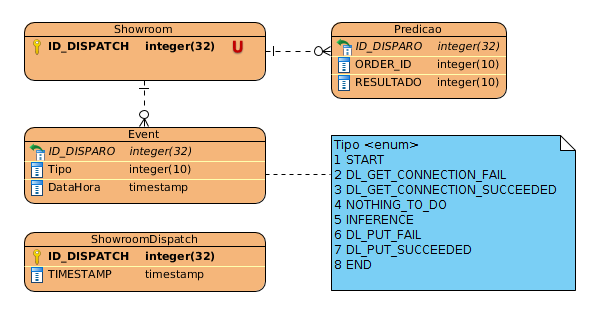
\includegraphics[scale=0.50]{ERD.png}
  \caption[\small{Diagrama Entidade-Relacionamento do banco.}]{\label{FigDel} \small{Diagrama Entidade-Relacionamento do banco.}}
  \end{center}
  }
\end{center}
\end{figure}

\begin{figure}
\begin{center}
\parbox[htb]{13.0cm}
  {
  \begin{center}
  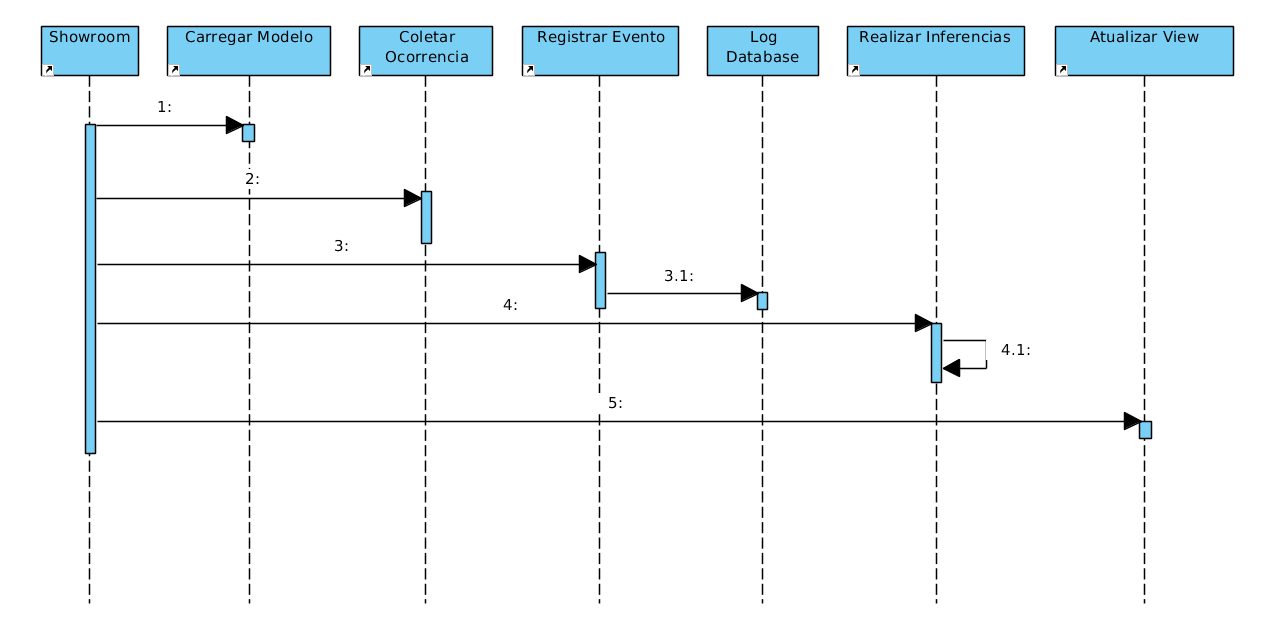
\includegraphics[scale=0.30]{sequence_showroom.png}
  \caption[\small{Diagrama de sequ�ncia da \textit{view Showroom}.}]{\label{FigDel} \small{Diagrama de sequ�ncia da \textit{view Showroom}.}}
  \end{center}
  }
\end{center}
\end{figure}

\subsection{Daemon}

\paragraph{}A componente \textit{daemon.py} se trata do \textit{script Python} respons�vel pelos disparos cuja execu��o � gerenciada pela aplica��o por meio do arquivo \textit{crontab}. A componente cont�m apenas um m�todo, o \textit{execute}, que � respons�vel por executar a predi��o de todos os casos dispon�veis no \textit{datalake}. Sua execu��o segue os passos do diagrama de sequ�ncia visto na figura 3.5. Inicialmente um novo disparo � inicializado e o evento de inicializa��o � armazenado no banco da aplica��o, o modelo de infer�ncia � carregado para mem�ria da aplica��o, as ocorr�ncias a sofrerem o processo preditivo s�o coletadas do \textit{datalake} e o evento de coleta � registrado. Ap�s isso as predi��es s�o realizadas e seus resultados s�o registrados no banco da aplica��o. Posteriormente, os resultados s�o salvos no \textit{datalake} e o evento de inser��o � salvo. Por fim, o evento de finaliza��o � armazenado.

\paragraph{}O disparo, os eventos e os resultados das predi��es das ocorr�ncias s�o armazenados no banco da aplica��o fazendo uso das entidades observadas na figura 3.3.

\begin{figure}
\begin{center}
\parbox[htb]{13.0cm}
  {
  \begin{center}
  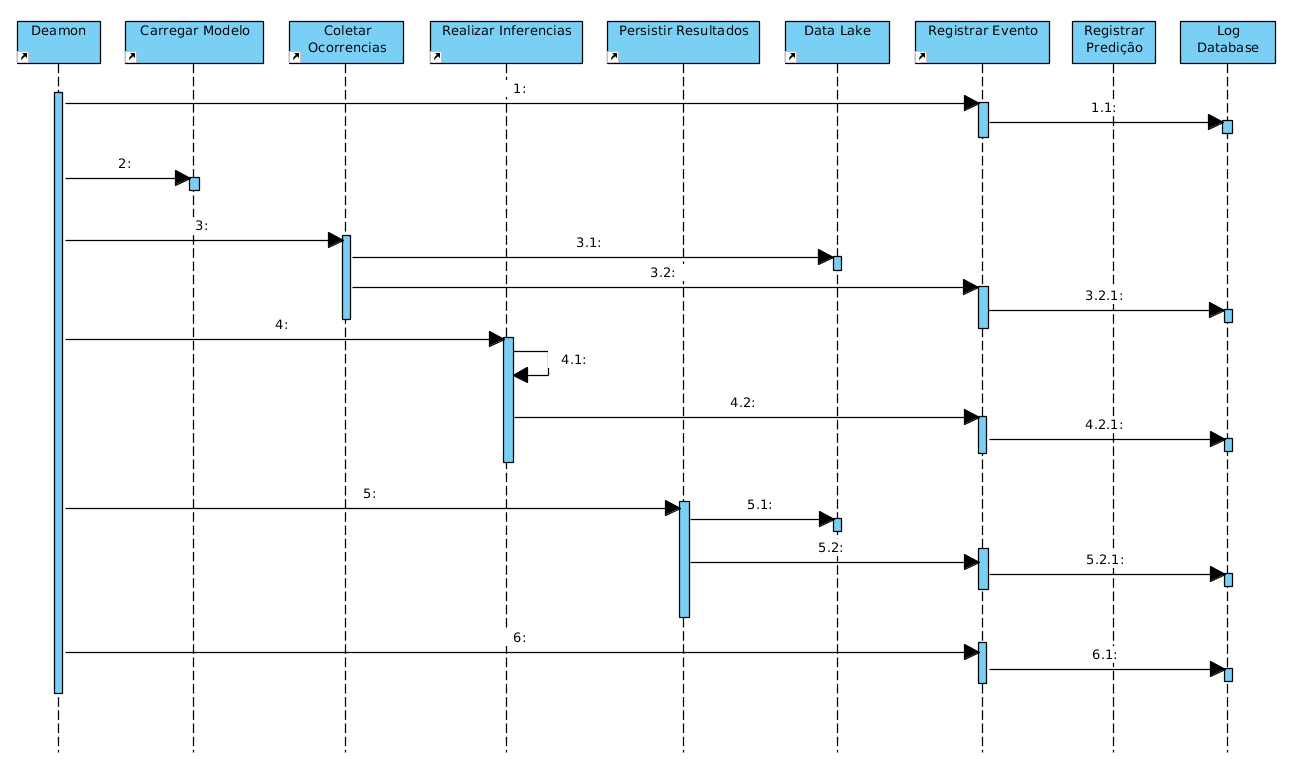
\includegraphics[scale=0.30]{sequence_daemon.png}
  \caption[\small{Diagrama de sequ�ncia da componente \textit{daemon.py}.}]{\label{FigDel} \small{Diagrama de sequ�ncia da \textit{view Showroom}.}}
  \end{center}
  }
\end{center}
\end{figure}

\subsection{Disparo}

\paragraph{} A \textit{view Disparo} � respons�vel por permitir a visualiza��o dos disparos executados, onde cada disparo � dado pela execu��o do script de infer�ncia. Nela � poss�vel visualizar todos os disparos executados pela componente \textit{daemon.py} a partir de um filtro temporal. Todos os resultados de todas as predi��es dentro do intervalo temporal selecionado s�o visualizados em tabelas, uma tabela para cada disparo. Os m�todos dessa componente podem ser vistos na tabela 3.5, referente � componente dispatch.py.

\begin{table}[]
\centering
\caption{M�todos do componente \textit{dispatch.py}.}
\label{dispatch}
\resizebox{\textwidth}{!}{%
\begin{tabular}{|l|l|}
\hline
M�todo                        & Descri��o                                                                                                                                                                                       \\ \hline
get\_dispatch\_events         & Retorna todos os eventos relacionados ao disparo com id igual ao fornecido                                                                                                                      \\ \hline
get\_dispatch\_predictions    & \begin{tabular}[c]{@{}l@{}}Retorna todos os resultados de predi��es relacionados ao disparo com id igual \\ ao fornecido\end{tabular}                                                           \\ \hline
get\_dispatches\_by\_interval & Retorna todos os ids dos disparos que ocorreram dentro de um intervalo temporal                                                                                                                 \\ \hline
to\_utc                       & \begin{tabular}[c]{@{}l@{}}Converte uma cadeia de caracteres no formato de hora e data \\ yyyy-MM-ddThh:mm:ss-hh:mm para um objeto datetime na zona UTC\end{tabular}                            \\ \hline
get\_last\_dispatches         & \begin{tabular}[c]{@{}l@{}}Retorna todos os eventos e resultados de predi��es para todos os disparos que \\ ocorreram entre as datas start e end, agrupados pelos ids dos disparos\end{tabular} \\ \hline
\end{tabular}%
}
\end{table}

\subsection{Monitor}

\paragraph{} A \textit{view Monitor} � respons�vel por monitorar: o estado de um \textit{host}, o estado do banco de dados, as datas dos �ltimo e pr�ximo disparos e o estado do escalonamento da componente \textit{daemon.py} a partir do arquivo \textit{crontab}. Em intervalos peri�dicos de tempo a \textit{view} � atualizada trazendo informa��es recentes para a interface, o que � feito por meio de uma requisi��o ass�ncrona chamada pela interface. A cada execu��o da atualiza��o, os m�todos \textit{get\_datalake\_status}, \textit{get\_process\_status}, \textit{get\_dispatch\_shedule}, \textit{get\_server\_status} e \textit{get\_db\_status} s�o executados pela componente \textit{view.py} e os resultados s�o enviados como resposta � requisi��o ass�ncrona, coforme visto no trecho de c�digo abaixo. Os m�todos dessa componente podem ser vistos na tabela 3.6.

\hfill \break
\lstset{language=Python}
\lstset{frame=lines}
%\lstset{caption={Insert code directly in your document}}
\lstset{label={lst:code_direct}}
\lstset{basicstyle=\footnotesize}
\begin{lstlisting}
def get_monitor_status(request):
    monitor = modules.Monitor()
    data = {
        'server': monitor.get_server_status(
        		settings.FRAMEWORK_CONFIG \
        		['monitor']['controller']['server']),
        'datalake': monitor.get_datalake_status(
         	settings.FRAMEWORK_CONFIG['datalake']),
        'process': monitor.get_process_status(
        		settings.FRAMEWORK_CONFIG),
        'visits': monitor.get_visits_datetimes(
        		settings.FRAMEWORK_CONFIG),
        'database': monitor.get_db_status(
        		settings.FRAMEWORK_CONFIG["mysql_events_db"])
    }
    return JsonResponse(data)
\end{lstlisting}

\paragraph{} Para a verifica��o do estado de um servidor, uma conex�o socket � criada em uma porta aberta qualquer do host. A conex�o � tida como \textit{offline} se ocorrer um timeout, sendo 10 segundos o intervalo de tempo para que isso ocorra. O host informado pode ser tanto como um endere�o IPV4 quanto um endere�o IPV6. Ainda � poss�vel monitorar servidores a partir de seu nome de dom�nio, mudando o mecanismo configurado de \textit{plain} ou \textit{ssl} para \textit{dns}, conforme visto no par�metro \textit{monitor.controller.server.mechanism} da tabela 3.1. O m�todo que realiza essa verifica��o pode ser visto abaixo.

\hfill \break
\lstset{language=Python}
\lstset{frame=lines}
%\lstset{caption={Insert code directly in your document}}
\lstset{label={lst:code_direct}}
\lstset{basicstyle=\footnotesize}
\begin{lstlisting}
def server_is_up(self,server):
     srv, mechanism, port = server
     try:
         if mechanism == 'plain':
             socket.create_connection(
          		(srv, port), timeout=10)
         elif mechanism == 'ssl':
             ssl.wrap_socket(
            		socket.create_connection(
            			("%s" % srv, port), timeout=10))
         elif mechanism == 'dns':
             host = socket.gethostbyname(srv)
             socket.create_connection(
            		(host, port), timeout=10)
         else:
             raise ValueError("Invalid mechanism")
         return ("online","")
     except socket.timeout:
         return ("offline","connection timeout")
     except Exception as err:
         return ("error", err.__str__())
\end{lstlisting}

\paragraph{} A verifica��o do estado do \textit{datalake} � feita por meio de uma conex�o, usando a cadeia de conex�o adequada ao banco a ser conectado. Ap�s a conex�o ser estabelecida, � realizada uma consulta simples em uma tabela qualquer pertencente ao banco, sem que nada seja retornado, com o intuito de que todos os passos da conex�o sejam testados. Caso ocorra algum problema em algum momento durante a tentativa de conex�o, esse problema � reportado. Essa l�gica pode ser vista no trecho de c�digo abaixo.

\hfill \break
\lstset{language=Python}
\lstset{frame=lines}
%\lstset{caption={Insert code directly in your document}}
\lstset{label={lst:code_direct}}
\lstset{basicstyle=\footnotesize}
\begin{lstlisting}
def get_datalake_status(self, datalake_settings):
    try:
        if self.datalake is None:
            self.datalake =
            	dl.Datalake(
            		datalake_settings["connection_string"])
        table = datalake_settings["table"]
    
        self.datalake.execute(
        	'SELECT * FROM {} LIMIT 1'.format(table))
    except pyodbc.Error as err:
        print(err)
            return { 'status': "error", 'error': str(err)}
        return { 'status': "online", 'error': ''}
\end{lstlisting}

\paragraph{} O �ltimo disparo e o estado do pr�ximo disparo s�o monitorados fazendo uso da biblioteca \textit{crontab} para \textit{Python 3}. Tanto a agenda de execu��es quanto o comando a ser executado pelo \textit{daemon cron} s�o obtidos por meio do uso dessa biblioteca. A verifica��o do estado do comando � feita como mostrado no trecho abaixo.

\hfill \break
\lstset{language=Python}
\lstset{frame=lines}
%\lstset{caption={Insert code directly in your document}}
\lstset{label={lst:code_direct}}
\lstset{basicstyle=\footnotesize}
\begin{lstlisting}
def get_process_status(self, config):
    try:
        expr = config['daemon']['cron']
        sheduler = CronTab(user=config['daemon']['user'])
        for job in sheduler:
            if job.comment == config['daemon']['comment']:
                if not job.is_valid():
                    return {"status": "invalid", "cron": expr, "error": ""}
                if not job.is_enabled():
                    return {"status": "disabled", "cron": expr, "error": ""}
                return {"status": "active", "cron": expr, "error": ""} 
        return {"status": "inactive", "cron": expr, "error": ""}
    except Exception as e:
        return {"status": "error", "cron": expr, "error":str(e)}
\end{lstlisting}

\paragraph{}Al�m de monitorar os servi�os associados ao \textit{framework}, a \textit{view} Monitor tamb�m � respons�vel pelo controle do estado do escalonamento da componente \textit{daemon.py}. Em sua interface, acess�vel apenas por administradores, � poss�vel adicionar e remover o comando de execu��o do \textit{script daemon.py} do arquivo \textit{crontab}, efetivamente controlando se a execu��o ocorrer� ou n�o conforme previsto pela express�o CRON presente no arquivo de configura��o no par�metro \textit{daemon.cron}, visto na tabela 3.1. Esse controle � feito por meio dos m�todos \textit{kill\_process} e \textit{start\_process}, vistos abaixo.

\hfill \break
\lstset{language=Python}
\lstset{frame=lines}
%\lstset{caption={Insert code directly in your document}}
\lstset{label={lst:code_direct}}
\lstset{basicstyle=\footnotesize}
\begin{lstlisting}
def kill_process(self,config):
    sheduler = CronTab(user=config['daemon']['user'])
    for job in sheduler:
        if job.comment == config['daemon']['comment']:
            sheduler.remove(job)
            sheduler.write()

def start_process(self, config):
    self.kill_process(config)
    cmd = '''{} "{}"'''.format(
    	config['daemon']['command'], config['path'])
    venv = config['daemon']['venv']
    if venv is not None and venv != "":
        cmd = "source {} ; {} ; deactivate".format(venv, cmd)
        cmd = '''"$(command -v bash)" -c '{}' '''.format(cmd)

    sheduler = CronTab(user=config['daemon']['user'])
    job = sheduler.new(command= cmd,
                        comment=config['daemon']['comment'])
    job.parse(config['daemon']['cron'])
\end{lstlisting}

\begin{table}[]
\centering
\caption{M�todos do componente \textit{monitor.py}.}
\label{monitor}
\resizebox{\textwidth}{!}{%
\begin{tabular}{|l|l|}
\hline
M�todo                  & Descri��o                                                                                                                                                                             \\ \hline
get\_datalake\_status   & Retorna o estado da conex�o com o datalake e o erro de conex�o, se houver                                                                                                             \\ \hline
get\_process\_status    & Retorna o estado do comando gerenciado no arquivo crontab                                                                                                                             \\ \hline
get\_dispatch\_schedule & \begin{tabular}[c]{@{}l@{}}Retorna a express�o CRON usada para agendar as execu��es do comando \\ gerenciado no arquivo crontab\end{tabular}                                          \\ \hline
kill\_process           & Remove o comando de execu��o do daemon do arquivo crontab                                                                                                                             \\ \hline
start\_process          & \begin{tabular}[c]{@{}l@{}}Inicia o agendamento do comando gerenciado no arquivo crontab, removendo\\ quaisquer comandos que possuam o mesmo id\end{tabular}                          \\ \hline
get\_server\_status     & Retorna o estado de um host, obtido a partir de conex�es criadas via sockets                                                                                                          \\ \hline
get\_db\_status         & \begin{tabular}[c]{@{}l@{}}Se conecta com o banco de dados da aplica��o gerenciado pelo Django e \\ retorna o estado da conex�o e o erro de conex�o, se houver\end{tabular}           \\ \hline
get\_visits\_datetimes  & \begin{tabular}[c]{@{}l@{}}Retorna a �ltima e pr�xima data de execu��o para o comando gerenciado no\\ arquivo crontab, se ativo. Retorna 'N/A' para ambas caso contr�rio\end{tabular} \\ \hline
server\_is\_up          & \begin{tabular}[c]{@{}l@{}}Verifica se um host est� online usando sockets e retorna seu estado e o erro \\ de conex�o, se houver\end{tabular}                                         \\ \hline
\end{tabular}%
}
\end{table}                 

\subsection{Urls}

\paragraph{}A componente \textit{urls.py} � respons�vel por descrever as rotas da aplica��o. Nela, os caminhos que levam �s \textit{views} e �s chamadas ass�ncronas est�o detalhadas em uma lista, fazendo a associa��o direta entre as fun��es da componete \textit{views.py} e as rotas usadas pelo usu�rio e pela interface da aplica��o. As rotas existentes podem ser vistas na tabela 3.7.

   

% Please add the following required packages to your document preamble:
% \usepackage{graphicx}
\begin{table}[]
caption{Rotas definidas na componente \textit{urls.py}.}
\label{urls}
\resizebox{\textwidth}{!}{%
\begin{tabular}{|l|l|}
\hline
Rota                             & Descri��o                                                                                                 \\ \hline
redirect/                        & Rota de redirecionamento ap�s o \textbackslash{}textit\{login\}                                           \\ \hline
monitor/                         & Rota para acesso � \textbackslash{}textit\{view\} Monitor                                                 \\ \hline
dispatch/                        & Rota para acesso � \textbackslash{}textit\{view\} Disparo                                                 \\ \hline
showroom/                        & Rota para acesso � \textbackslash{}textit\{view\} Showroom                                                \\ \hline
dispatch/update\_dispatch/       & Rota para requisi��o ass�ncrona de atualiza��o da \textbackslash{}textit\{view\} Disparo                  \\ \hline
showroom/update\_showroom/       & Rota para requisi��o ass�ncrona de atualiza��o da \textbackslash{}textit\{view\} Showroom                 \\ \hline
showroom/update\_showroom\_item/ & Rota para requisi��o ass�ncrona de atualiza��o de um dos items da \textbackslash{}textit\{view\} Showroom \\ \hline
monitor/monitor\_status/         & Rota para requisi��o ass�ncrona de atualiza��o  da \textbackslash{}textit\{view\} Monitor                 \\ \hline
monitor/process\_kill/           & Rota para requisi��o ass�ncrona de remo��o do comando no arquivo \textbackslash{}textit\{crontab\}        \\ \hline
monitor/process\_start/          & Rota para requisi��o ass�ncrona de inser��o do  comando no arquivo \textbackslash{}textit\{crontab\}      \\ \hline
\end{tabular}%
}
\end{table}

\section{Implanta��o}

\begin{figure}
\begin{center}
\parbox[htb]{13.0cm}
  {
  \begin{center}
  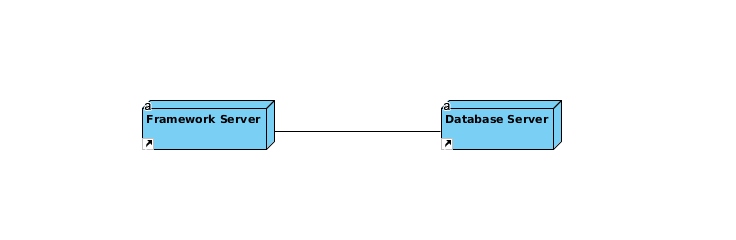
\includegraphics[scale=0.50]{deployment.png}
  \caption[\small{Diagrama de implanta��o.}]{\label{FigDel} \small{Diagrama de implanta��o}}
  \end{center}
  }
\end{center}
\end{figure}

\subsection{Configura��o do ambiente}

\paragraph{}Para configura�ao do ambiente, o primeiro passo � sua obten��o, que, para o caso da implanta��o desse projeto, foi obtido por meio do aluguel de um servidor da \textit{Amazon AWS}. O segudo � a obten��o do c�digo fonte, que se encontra hospedado em um reposit�rio do servi�o \textit{Github}. Com o uso de uma conta autorizada a ter acesso ao reposit�rio, � preciso realizar o download do projeto. Posteriormente, � necess�rio seguir as instru��es presentes no arquivo \textit{README.md}, que cont�m detalhados todos os passos necess�rios para a configura��o do ambiente.

\paragraph{}O primeiro � preparar o ambiente \textit{Python 3}, instalando a linguagem no servidor em que ser� executada a aplica��o. Em seguida, � necess�rio criar um ambiente virtual e instalar nele todas as depend�ncias da aplica��o fazendo uso do arquivo \textit{requirements.txt}. Enfim, � preciso preparar o ambiente \textit{Django}, criando os usu�rios e grupos descritos no arquivo \textit{README.md}. 

\paragraph{}Ap�s isso, � necess�rio instalar e configurar o banco da aplica��o em algum servidor acess�vel ao servidor da aplica��o, ou no mesmo servidor. Para isso, deve-se instalar o banco de dados MySQL, criar um usu�rio e \textit{database} para uso da aplica��o e executar o comando do \textit{framework Django} que cria as tabelas a partir dos arquivos do projeto.

\paragraph{}Para a conex�o com o \textit{datalake}, � preciso instalar o conector \textit{ODBC} compat�vel com o tipo de banco de dados usado pelo \textit{datalake} no servidor da aplica��o. Por fim, � preciso configurar os par�metros da aplica��o contidos no arquivo \textit{config.yaml}, que se encontra no diret�rio raiz do projeto, conforme visto na tabela 3.1.



\subsection{Inicializa��o da aplica��o}

\paragraph{}Para a inicializa��o da aplica��o, basta certificar-se de que o banco da aplica��o est� operacional e executar o comando que inicia a  execu��o da aplica��o \textit{Django}, conforme visto no arquivo \textit{README.md}.

% ---------------------------------------------------------------
% Chapter 4 - Conclusoes
% ---------------------------------------------------------------
\chapter{Conclus�es}
\label{cap4}
\section{TODO}



% ---------------------------------------------------------------
% Bibliografia
% ---------------------------------------------------------------
\normalsize
\cleardoublepage
\addcontentsline{toc}{chapter}{Bibliografia}
\bibliographystyle{coppe}
\bibliography{biblio}

% ---------------------------------------------------------------
% Ap�ndices 
% ---------------------------------------------------------------
   %\appendix
   % ---------------------------------------------------------------
   % Ap�ndice A
   % ---------------------------------------------------------------
   %\chapter{O que � um ap�ndice}
   %\label{ApendiceA}
   %\paragraph{}Elemento que consiste em um texto ou documento elaborado pelo autor, com o intuito de complementar sua argumenta��o, sem preju�zo do trabalho. S�o identificados por letras mai�sculas consecutivas e pelos respectivos t�tulos.
   % ---------------------------------------------------------------
   % Ap�ndice B
   % ---------------------------------------------------------------
   %\chapter{Encaderna��o do Projeto de Gradua��o}
   %\label{ApendiceB}
   %\begin{figure}
\begin{center}
\parbox[htb]{13.0cm}
  {
  \begin{center}
  
\includegraphics[scale=1.0]{Capa_do_Projeto_Final.eps}
  \caption[\small{Encaderna��o do projeto de gradua��o.}]{\label{FigPFC} \small{Encaderna��o do projeto de gradua��o.}}
  \end{center}
  }
\end{center}
\end{figure}
   % ---------------------------------------------------------------
   % Ap�ndice C
   % ---------------------------------------------------------------
   %\chapter{O que � um anexo}
   %\label{ApendiceC}
   %\paragraph{}Documenta��o n�o elaborada pelo autor, ou elaborada pelo autor mas constituindo parte de outro projeto.   

\backmatter

\end{document}
